\documentclass[titlepage,a4paper]{article}

\usepackage{a4wide}
\usepackage[colorlinks=true,linkcolor=black,urlcolor=blue,bookmarksopen=true]{hyperref}
\usepackage{bookmark}
\usepackage{fancyhdr}
\usepackage[spanish]{babel}
\usepackage[utf8]{inputenc}
\usepackage[T1]{fontenc}
\usepackage{graphicx}
\usepackage{float}
\usepackage{listings}
\usepackage[table,xcdraw]{xcolor}
\usepackage{pdfpages}
\newcommand{\codigoMateria}{86.37 / 66.20}
\newcommand{\nombreMateria}{[86.37 / 66.20] Organización de Computadoras}
\newcommand{\curso}{2}
\usepackage{mips}
\usepackage{amssymb, amsmath, amsbsy} % librerias ams
\usepackage{cprotect}

\newcommand{\numeroTP}{0}
\newcommand{\tituloTP}{Trabajo práctico 2}
\newcommand{\descripcionTP}{Memoria Caché}

\newcommand{\facultad}{Facultad de Ingeniería}
\newcommand{\universidad}{Universidad de Buenos Aires}
\newcommand{\cuatrimestre}{2do Cuatrimestre de 2020}


\pagestyle{fancy} % Encabezado y pie de página
\fancyhf{}
\fancyhead[L]{TP2 - Memoria Caché}
\fancyhead[R]{Organización de Computadoras - FIUBA}
\renewcommand{\headrulewidth}{0.4pt}
\fancyfoot[C]{\thepage}
\renewcommand{\footrulewidth}{0.4pt}

\newcommand{\teammember}[3]{
	 #1 & #2 & \texttt{#3}\\
}

\begin{document}
\begin{titlepage} % Carátula
    \centering
      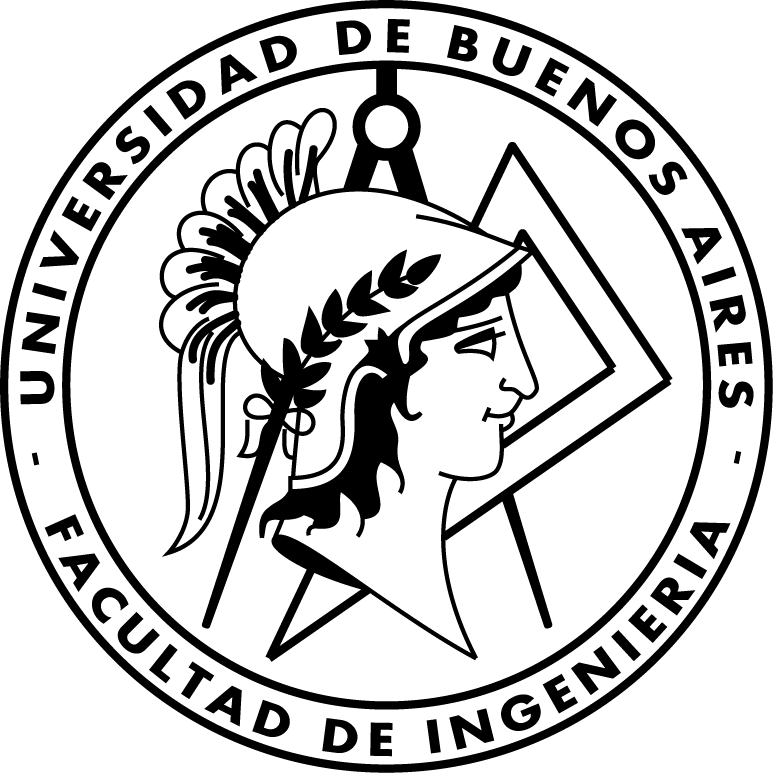
\includegraphics[scale = 0.75]{images/logo_fiuba.png}\\[1.0 cm]	% Logo universidad
      \textsc{\LARGE \universidad}\\[0.5 cm]	% Nombre universidad
      \textsc{\Large \facultad}\\[0.5 cm]	% Facultad
      \textsc{\large \cuatrimestre}\\[1.0 cm]	% Cuatrimestre
    \centering
    
     \textsc{\Large \nombreMateria}\\[0.5 cm] % Nombre materia
      \textsc{\large Curso \curso}\\[0.4 cm]	% Curso
      
      \rule{\linewidth}{0.2 mm} \\[0.4 cm]
      { \huge \tituloTP}\\[0.5 cm]
      { \huge \bfseries}
      { \huge \bfseries \descripcionTP}\\
      \rule{\linewidth}{0.2 mm} \\[1 cm]
      
      
     \resizebox{12cm}{!}{
        \begin{tabular}{ | c | l | l | }
          \hline
          Padrón & Alumno & Email \\
          \hline
          \teammember{103442}{Lovera, Daniel}{dlovera@fi.uba.ar}
          \teammember{102914}{More, Agustín}{amore@fi.uba.ar}
          \teammember{99846}{Torresetti, Lisandro}{ltorresetti@fi.uba.ar}
          \hline
      	\end{tabular}
  	}
  	\vskip2cm
  	\Large Repositorio: \url{https://github.com/DanieLovera/Orga}
  	
\end{titlepage}


\tableofcontents % Índice general
\newpage

\lstdefinestyle{customC}{
  language=C,                % choose the language of the code
  backgroundcolor=\color[HTML]{fcfbfc},
  numbers=left,                   % where to put the line-numbers
  stepnumber=1,                   % the step between two line-numbers.        
  numbersep=10pt,                  % how far the line-numbers are from the code
  frame=l,	                   % adds a frame around the code
  showspaces=false,               % show spaces adding particular underscores
  showstringspaces=false,         % underline spaces within strings
  keywordstyle=\color[HTML]{6684e1},
  stringstyle=\color[HTML]{1fad83},     % string literal style
  commentstyle=\color[HTML]{999580},
  showtabs=false,                 % show tabs within strings adding particular underscores
  tabsize=2,                      % sets default tabsize to 2 spaces
  captionpos=b,                   % sets the caption-position to bottom
  breaklines=true,                % sets automatic line breaking
  breakatwhitespace=true,         % sets if automatic breaks should only happen at whitespace
  title=\lstname,                 % show the filename of files included with \lstinputlisting;
  postbreak=\mbox{\textcolor{darkgray}{$\hookrightarrow$}\space},
}

\section{Objetivos}\label{sec:objetivos}
El trabajo práctico consiste en la simulación del comportamiento de una memoria caché asociativa por conjuntos, bajo la política \verb|LRU|, bajo la política de escritura \verb|WB/WA|.

\section{Introducción}\label{sec:intro}
La finalidad de una memoria caché consiste en reducir la cantidad de accesos de lecturas y escrituras de la memoria principal, poniéndose como intermediario entre la memoria principal y la \verb|CPU|. Al tratarse de una memoria que es menor a la memoria principal, existirán colisiones que deben manejarse. Particularmente, para el presente trabajo se cuenta con las políticas reemplazo \verb|LRU| (\textit{Least Recently Used}), que al momento de reemplazar algún registro, se reemplazará el que menos se haya solicitado últimamente. Luego, para la política de escritura, se utiliza \verb|WB/WA| (\textit{Write-Back/Write-Allocate}), es decir, cuando se tiene que escribir, primero se escribe en la memoria caché, y cuando sea necesario reemplazar ese registro de la caché, se escribirá finalmente en la memoria principal.

%\section{Programa a implementar}\label{sec:programa_a_implementar}
%Utilizando el lenguaje `C' se implementa un codificador y %decodificador de texto en base64. La entrada será un archivo %especificado en el comando o el \textit{stdin} si ninguno es %especificado, y la salida será otro archivo también especificado en %el comando o el \textit{stdout} si ninguno es especificado.

\section{Detalles de implementación}\label{sec:detalles_implementacion}
\subsection{Address Parser}
    Este módulo fue diseñado con la intención de que sea el encargado de convertir una dirección de memoria en cada campo especifico de la memoria caché \textbf{tag, set, offset}.
    \\ La interfaz del usuario queda definida como:
    \begin{lstlisting}[style=customC]
    unsigned int address_parser_tag(unsigned int address
	        , unsigned int block_size, unsigned int total_sets);
    unsigned int address_parser_set(unsigned int address
        	, unsigned int block_size, unsigned int total_sets);
    unsigned int address_parser_offset(unsigned int address
        	, unsigned int block_size);
    \end{lstlisting}
    En donde cada función devuelve el valor del campo correspondiente

\subsection{Memory}
    El módulo de memoria simula ser la memoria principal con un arreglo de caracteres de tamaño \textbf{64 Kb}, además implementa las operaciones de lectura y escritura necesarias. Las funciones mas importantes correspondientes a este modulo son:
    \begin{lstlisting}[style=customC]
    void memory_write(memory_t *self, char *data
	    	, int address, unsigned int data_size); 
    void memory_read(memory_t *self, char *data_buffer
	    	, int address, unsigned int data_size);
    \end{lstlisting}
    \begin{itemize}
        \item La función \textbf{memory\_write}  escribe un bloque entero de datos en memoria, para eso requiere recibir los datos, y la dirección de inicio en donde se van a escribir, el tamaño de los datos determina cuantos datos se van a copiar.
        \item La función \textbf{memory\_read}  es análoga a la anterior con la salvedad que recibe un buffer en donde se van a guardar los datos que hayan sido leídos de memoria.
    \end{itemize}

\subsection{Cache}
    Es finalmente el módulo mas importante para la simulación de la memoria caché SA/LRU, se utilizan el \textbf{Address parser} y \textbf{Memory} para completar el programa principal. 
    \\\\\indent A su vez la cache esta compuesta de dos estructuras de datos más pequeñas \textbf{struct set} y \textbf{struct block}, y se hace uso de memoria dinámica para poder implementar una cache que cambie dinámicamente dependiendo de la elección del usuario. Se define La interfaz del usuario como:
    
    \begin{lstlisting}[style=customC]
    void cache_init(unsigned int capacity, unsigned int ways_number,         unsigned int block_size);
    void cache_uninit();
    void init();
    unsigned int find_set(int address);
    unsigned int find_lru(int setnum);
    unsigned int is_dirty(int way, int setnum);
    void read_block(int blocknum);
    void write_block(int way, int setnum);
    char read_byte(int address);
    void write_byte(int address, char value);
    int get_miss_rate();
    \end{lstlisting}
    
    \subsubsection{Funciones importantes de implementación de cache.}
    \begin{itemize}
        \item La implementación de la política LRU se realizo en la función \textbf{find\_lru}, para ello cada bloque de memoria cache cuenta con un campo llamado \textbf{lru\_counter} el cual cada vez que es accedido es aumentado en una unidad si el campo \textbf{last\_used} lo permite. Por lo tanto para determinar cual es el bloque menos recientemente usado se compara linealmente el \textbf{lru\_counter} de cada bloque del set y se selecciona el menor de ellos, esto quiere decir que al ser el menos recientemente utilizado sera el bloque a reemplazar.
        \item Las lecturas a memoria cache se realizan en la función \textbf{read\_byte}, primero se descomponen los campos de tag y set del address y se realiza una búsqueda interna en cache para verficar si esta o no el bloque cargado. 
        \begin{itemize}
            \item En caso de que el dato este en cache simplemente se devuelve el dato como resultado.
            \item Si el dato no esta en cache, automáticamente se pasa a cargar el bloque desde memoria utilizando la función \textbf{read\_block} y luego se repite el llamado a la función \textbf{read\_byte} para buscar nuevamente el dato que esta vez estará cargado en cache
        \end{itemize}
        \item Las escrituras en memoria cache se realizan con la función \textbf{write\_byte} y el algoritmo de escritura es similar al de lectura, primero se realiza una búsqueda en cache del dato descomponiendo la dirección de memoria en los campos de cache necesarios.
            \begin{itemize}
                \item En caso de que el dato este en cache simplemente se escribe el dato en cache y se deja desactualizada la memoria.
                \item Si el dato no esta en cache, automáticamente se pasa a cargar el bloque desde memoria utilizando la función \textbf{read\_block} y luego se repite el llamado a la función \textbf{write\_byte} para buscar nuevamente el dato que esta vez estará cargado en cache.
        \end{itemize}
        \item Las lecturas de bloques de memoria principal a memoria cache se realizan con la función \textbf{read\_block}, la cual se encarga de leer los datos necesarios accediendo a memoria, pero antes de que sean guardados en cache verifica que el bloque no este sucio, si esto es así primero tiene que escribir ese bloque de cache en memoria antes de que sea sobreescrito llamando a la función \textbf{write\_block}. Una vez que el bloque sea llevado a memoria para actualizarse en caso de que estuviera sucio entonces se procede a leer el bloque correspondiente de memoria y cargarlo en cache.
        \item Las escrituras de bloques de memoria cache a memoria principal se realizan con la función \textbf{write\_block}, la cual únicamente se encarga de copiar el bloque entero a memoria luego de descomponer la dirección.
        \item El miss rate se calcula con la función \textbf{get\_miss\_rate} se encarga de calcular el miss rate de la memoria cache, para ello se cuenta con un campo interno en cache que cuenta la cantidad de misses y hits por accesos a cache (lecturas y escrituras), que son aumentados cada vez que se tiene que ir a buscar un dato a memoria o no.
    \end{itemize}
    
\section{Compilación y ejecución}

\subsection{Compilación}
Para compilar el programa implementado se incluyo un archivo \verb|Makefile|   en el repositorio, se debe ejecutar el comando \verb|make| \cite{makefile}, esto generará el archivo ejecutable \verb|main|.


En caso que se requiera limpiar automáticamente el \verb|build| realizado se puede ejecutar el comando \verb|make clean|, y removerá todos los archivos generados por el comando \verb|make|.

\subsection{Ejecución}
Para ejecutar el archivo compilado:
\begin{verbatim}
    ./main [Opciones] [archivo-de-entrada]
\end{verbatim}

\subsubsection{Descripción de parámetros}
\begin{itemize}
    \cprotect\item[\verb|-V|] {-}{-}version: Muestra la versión y sale del programa.
    \cprotect\item[\verb|-h|] {-}{-}help: Muestra información de ayuda de cómo ejecutar el programa y sale del programa.
    \cprotect\item[\verb|-o|] {-}{-}output: Path para el archivo de salida (opcionalmente, se puede obviar este parámetro e indicarlo como el último parámetro de la línea de comandos).
    \cprotect\item[\verb|-w|] {-}{-}ways: Cantidad de vías.
    \cprotect\item[\verb|-cs|] {-}{-}cachesize: Tamaño de la caché en kilobytes.
    \cprotect\item[\verb|-bs|] {-}{-}blocksize: Tamaño de bloque en bytes.
\end{itemize}

\subsubsection{Ejemplos de ejecución}

Para poder ejecutar el simulador, se deben pasar las características de la memoria caché (\textit{ways}, \textit{cachesize} y \textit{blocksize}). 


El siguiente ejemplo simulará la ejecución de las instrucciones que se encuentran en \verb|prueba1.mem| sobre una caché de 4 vías, de tamaño de 8 KB y de tamaño de bloque 16 bytes.

\begin{verbatim}
    ./tp2 -w 4 -cs 8 -bs 16 prueba1.mem
\end{verbatim}

Otra manera de ejecutar la misma línea, sin importar el orden de los parámetros, es mediante el comando:
\begin{verbatim}
    ./tp2 -w 4 -cs 8 -bs 16 -o prueba1.mem
\end{verbatim}

\section{Pruebas}
\lstdefinestyle{test_run_style}{
    breaklines=true,
    breakatwhitespace=false,
    postbreak=\mbox{\textcolor{darkgray}{$\hookrightarrow$}\space},
    frame=single,
    framesep=10pt
}

\subsection{Pruebas de la cátedra}

La cátedra presenta dos casos de pruebas sobre dos configuraciones de memoria caché distintas:
\begin{itemize}
    \item Caché 1:
    \begin{itemize}
        \item 4KB tamaño de caché.
        \item 4 vías.
        \item 32 bytes tamaño del bloque.
    \end{itemize}
    \item Caché 2:
    \begin{itemize}
        \item 16KB tamaño de caché.
        \item 1 vía.
        \item 128 bytes tamaño del bloque.
    \end{itemize}
\end{itemize}

Los dos casos de pruebas son sobre las siguentes secuencias:

\begin{itemize}
    \item Secuencia 1 (\verb|prueba1.mem|):
    \begin{verbatim}
    init
    W 0, 255
    W 16384, 254
    W 32768, 248
    W 49152, 096
    R 0
    R 16384
    R 32768
    R 49152
    MR
    \end{verbatim}
    \item Secuencia 2 (\verb|prueba2.mem|):
    \begin{verbatim}
    init
    W 0, 123
    W 1024, 234
    W 2048, 33
    W 3072, 44
    W 4096, 55
    R 0
    R 1024
    R 2048
    R 3072
    R 4096
    MR
    \end{verbatim}
\end{itemize}

Las ejecuciones de estas simulaciones serán para la secuencia 1 (\verb|prueba1.mem|):

\begin{itemize}
    \item En la caché 1:
    
    \begin{itemize}
        \item Comando: \verb|./main -cs 4 -w 4 -bs 32 prueba1.mem|
        \item Salida:
            \begin{verbatim}
        Se inicia la caché
        Escribe � en la dirección 0
        Escribe � en la dirección 16384
        Escribe � en la dirección 32768
        Escribe ` en la dirección 49152
        Leo de la dirección 0 y obtengo �
        Leo de la dirección 16384 y obtengo �
        Leo de la dirección 32768 y obtengo �
        Leo de la dirección 49152 y obtengo `
        MR: %50
            \end{verbatim}
    \end{itemize}
    
    \item En la caché 2:
    \begin{itemize}
        \item Comando: ``` ./main -cs 16 -w 1 -bs 128 prueba1.mem ```
        \item Salida:
            \begin{verbatim}
        Se inicia la caché
        Escribe � en la dirección 0
        Escribe � en la dirección 16384
        Escribe � en la dirección 32768
        Escribe ` en la dirección 49152
        Leo de la dirección 0 y obtengo �
        Leo de la dirección 16384 y obtengo �
        Leo de la dirección 32768 y obtengo �
        Leo de la dirección 49152 y obtengo `
        MR: %100
            \end{verbatim}
    \end{itemize}
\end{itemize}

Las ejecuciones de estas simulaciones serán para la secuencia 2 (\verb|prueba2.mem|):

\begin{itemize}
    \item En la caché 1:
    \begin{itemize}
        \item Comando: \verb|./main -cs 4 -w 4 -bs 32 prueba2.mem|
        \item Salida:
            \begin{verbatim}

        Se inicia la caché
        Escribe { en la dirección 0
        Escribe � en la dirección 1024
        Escribe ! en la dirección 2048
        Escribe , en la dirección 3072
        Escribe 7 en la dirección 4096
        Leo de la dirección 0 y obtengo {
        Leo de la dirección 1024 y obtengo �
        Leo de la dirección 2048 y obtengo !
        Leo de la dirección 3072 y obtengo ,
        Leo de la dirección 4096 y obtengo 7
        MR: %70
            \end{verbatim}

    \end{itemize}
    
    \item En la caché 2:
    \begin{itemize}
        \item Comando: \verb|./main -cs 16 -w 1 -bs 128 prueba2.mem|
        \item Salida:
            \begin{verbatim}
    Se inicia la caché
    Escribe { en la dirección 0
    Escribe � en la dirección 1024
    Escribe ! en la dirección 2048
    Escribe , en la dirección 3072
    Escribe 7 en la dirección 4096
    Leo de la dirección 0 y obtengo {
    Leo de la dirección 1024 y obtengo �
    Leo de la dirección 2048 y obtengo !
    Leo de la dirección 3072 y obtengo ,
    Leo de la dirección 4096 y obtengo 7
    MR: %50
            \end{verbatim}
    \end{itemize}
\end{itemize}




\subsection{Pruebas propias}
Las pruebas propias se encuentran en la carpeta 'pruebas' y van desde la 'prueba3.mem' a la 'prueba6.mem'. Para ejecutar las pruebas se utilizó el siguiente comando:
$$\verb|./main -cs 4 -w 4 -bs 32 pruebaX.mem|, \quad  X = 3,4,5,6$$
A continuación se muestra el contenido de cada prueba y su respectiva salida.\\

\begin{itemize}
    \item Prueba 3:
    \begin{itemize}
        \item Contenido:
            \begin{verbatim}
                init
                W 0, 0
                W 1, 65
                R 0
                R 1
                W 32, 71
                R 32
                W 16, 90
                W 0, 67
                R 0
                MR
            \end{verbatim}
        \item Salida:
            \begin{verbatim}
                Se inicia la caché
                Escribe  en la dirección 0
                Escribe A en la dirección 1
                Leo de la dirección 0 y obtengo 
                Leo de la dirección 1 y obtengo A
                Escribe G en la dirección 32
                Leo de la dirección 32 y obtengo G
                Escribe Z en la dirección 16
                Escribe C en la dirección 0
                Leo de la dirección 0 y obtengo C
                MR: %22
            \end{verbatim}
    \end{itemize}
    \item Prueba 4:
    \begin{itemize}
        \item Contenido:
            \begin{verbatim}
                init
                W 65535, 77
                W 65534, 78
                W 65533, 79
                W 32768, 65
                W 32768, 66
                R 65535
                R 65534
                R 65533
                R 32768
                R 65535
                MR
            \end{verbatim}
        \item Salida:
            \begin{verbatim}
                Se inicia la caché
                Escribe M en la dirección 65535
                Escribe N en la dirección 65534
                Escribe O en la dirección 65533
                Escribe A en la dirección 32768
                Escribe B en la dirección 32768
                Leo de la dirección 65535 y obtengo M
                Leo de la dirección 65534 y obtengo N
                Leo de la dirección 65533 y obtengo O
                Leo de la dirección 32768 y obtengo B
                Leo de la dirección 65535 y obtengo M
                MR: %20
            \end{verbatim}
    \end{itemize}
    \item Prueba 5:
    \begin{itemize}
        \item Contenido:
            \begin{verbatim}
                init
                R 0
                W 0, 65
                W 1, 66
                W 2, 67
                R 0
                R 1
                R 2
                MR
            \end{verbatim}
        \item Salida:
            \begin{verbatim}
                Se inicia la caché
                Leo de la dirección 0 y obtengo 
                Escribe A en la dirección 0
                Escribe B en la dirección 1
                Escribe C en la dirección 2
                Leo de la dirección 0 y obtengo A
                Leo de la dirección 1 y obtengo B
                Leo de la dirección 2 y obtengo C
                MR: %14
            \end{verbatim}
    \end{itemize}
    \item Prueba 6:
    \begin{itemize}
        \item Contenido:
            \begin{verbatim}
                init
                W 0, 65
                W 1, 66
                W 2, 67
                W 3, 68
                W 4, 69
                W 5, 70
                W 6, 71
                W 7, 72
                W 8, 73
                W 9, 74
                W 10, 75
                W 11, 76
                W 12, 77
                W 13, 78
                W 14, 79
                W 15, 80
                W 16, 81
                W 17, 82
                W 18, 83
                W 19, 84
                W 20, 85
                W 21, 86
                W 22, 87
                W 23, 88
                W 24, 89
                W 25, 90
                W 26, 91
                R 0
                R 1
                R 2
                R 3
                R 4
                R 5
                R 6
                R 7
                R 8
                R 9
                R 10
                R 11
                R 12
                R 13
                R 14
                R 15
                R 16
                R 17
                R 18
                R 19
                R 20
                R 21
                R 22
                R 23
                R 24
                R 25
                R 26
                MR
            \end{verbatim}
        \item Salida:
            \begin{verbatim}
                Se inicia la caché
                Escribe A en la dirección 0
                Escribe B en la dirección 1
                Escribe C en la dirección 2
                Escribe D en la dirección 3
                Escribe E en la dirección 4
                Escribe F en la dirección 5
                Escribe G en la dirección 6
                Escribe H en la dirección 7
                Escribe I en la dirección 8
                Escribe J en la dirección 9
                Escribe K en la dirección 10
                Escribe L en la dirección 11
                Escribe M en la dirección 12
                Escribe N en la dirección 13
                Escribe O en la dirección 14
                Escribe P en la dirección 15
                Escribe Q en la dirección 16
                Escribe R en la dirección 17
                Escribe S en la dirección 18
                Escribe T en la dirección 19
                Escribe U en la dirección 20
                Escribe V en la dirección 21
                Escribe W en la dirección 22
                Escribe X en la dirección 23
                Escribe Y en la dirección 24
                Escribe Z en la dirección 25
                Escribe [ en la dirección 26
                Leo de la dirección 0 y obtengo A
                Leo de la dirección 1 y obtengo B
                Leo de la dirección 2 y obtengo C
                Leo de la dirección 3 y obtengo D
                Leo de la dirección 4 y obtengo E
                Leo de la dirección 5 y obtengo F
                Leo de la dirección 6 y obtengo G
                Leo de la dirección 7 y obtengo H
                Leo de la dirección 8 y obtengo I
                Leo de la dirección 9 y obtengo J
                Leo de la dirección 10 y obtengo K
                Leo de la dirección 11 y obtengo L
                Leo de la dirección 12 y obtengo M
                Leo de la dirección 13 y obtengo N
                Leo de la dirección 14 y obtengo O
                Leo de la dirección 15 y obtengo P
                Leo de la dirección 16 y obtengo Q
                Leo de la dirección 17 y obtengo R
                Leo de la dirección 18 y obtengo S
                Leo de la dirección 19 y obtengo T
                Leo de la dirección 20 y obtengo U
                Leo de la dirección 21 y obtengo V
                Leo de la dirección 22 y obtengo W
                Leo de la dirección 23 y obtengo X
                Leo de la dirección 24 y obtengo Y
                Leo de la dirección 25 y obtengo Z
                Leo de la dirección 26 y obtengo [
                MR: %1
            \end{verbatim}
    \end{itemize}
\end{itemize}


% \begin{lstlisting}[style=test_run_style]
% ./common --divisor 10 -10

% Error: Numero fuera de rango [2, 2147483647).

% \end{lstlisting}

\section{Conclusiones}
    Se implemento una memoria cache LRU, es decir la política de reemplazo fue modificar el bloque de cache menos recientemente utilizado, la política de reemplazo es necesaria en caches que tengan algún grado de asociatividad pues el mapeo de un bloque de memoria a uno de cache no es uno a uno, esto lleva a la necesidad de una política de reemplazo. Adicionalmente cuando se escribe un dato en memoria se requiere evaluar una política de escritura, en este caso se implemento la política write back/write allocate, por lo cual ante un miss en escritura, el programa levanta un bloque de memoria principal y lo guarda en cache, para posteriormente ser escrito como si el cache siempre hubiese tenido ese dato, y ante un hit en escritura el programa escribe directamente sobre memoria cache y deja desactualizada la memoria principal, hasta que un bloque de memoria cache tenga que ser reemplazado, en cuyo caso el programa primero baja el bloque a memoria principal para actualizarlo y posteriormente escribe el nuevo bloque en cache.
    \\\\\indent Según las pruebas ejecutadas vemos la tasa de miss de la memoria cache depende de como esta este conformada, ya que en la prueba1.mem provista por la cátedra la tasa de miss de una cache grande con un menor grado de asociatividad y un tamaño de bloque mayor genera una tasa de miss de 100\%, y en la prueba2.mem se observa una tasa de miss de 50\% es decir menor a la prueba de cache para una memoria mas pequeña de menor grado de asociatividad y un tamaño de bloque menor.


\newpage
\appendix
\section{Código}
\subsection{Código en C}
\label{apendice:codigo_c}
\subsubsection{main.c}
\lstinputlisting[style=customC]{code/main.c}

\subsubsection{cache.c}
\lstinputlisting[style=customC]{code/cache.c}

\subsubsection{cache.h}
\lstinputlisting[style=customC]{code/cache.h}

\subsubsection{memory.c}
\lstinputlisting[style=customC]{code/memory.c}

\subsubsection{memory.h}
\lstinputlisting[style=customC]{code/memory.h}

\subsubsection{address_parser.c}
\lstinputlisting[style=customC]{code/address_parser.c}

\subsubsection{address_parser.h}
\lstinputlisting[style=customC]{code/address_parser.h}

\subsubsection{parsers.c}
\lstinputlisting[style=customC]{code/parsers.c}

\subsubsection{parsers.h}
\lstinputlisting[style=customC]{code/parsers.h}

\subsubsection{strutil.c}
\lstinputlisting[style=customC]{code/strutil.c}

\subsubsection{strutil.h}
\lstinputlisting[style=customC]{code/strutil.h}


% \newpage
\section{Enunciado del trabajo práctico}
% 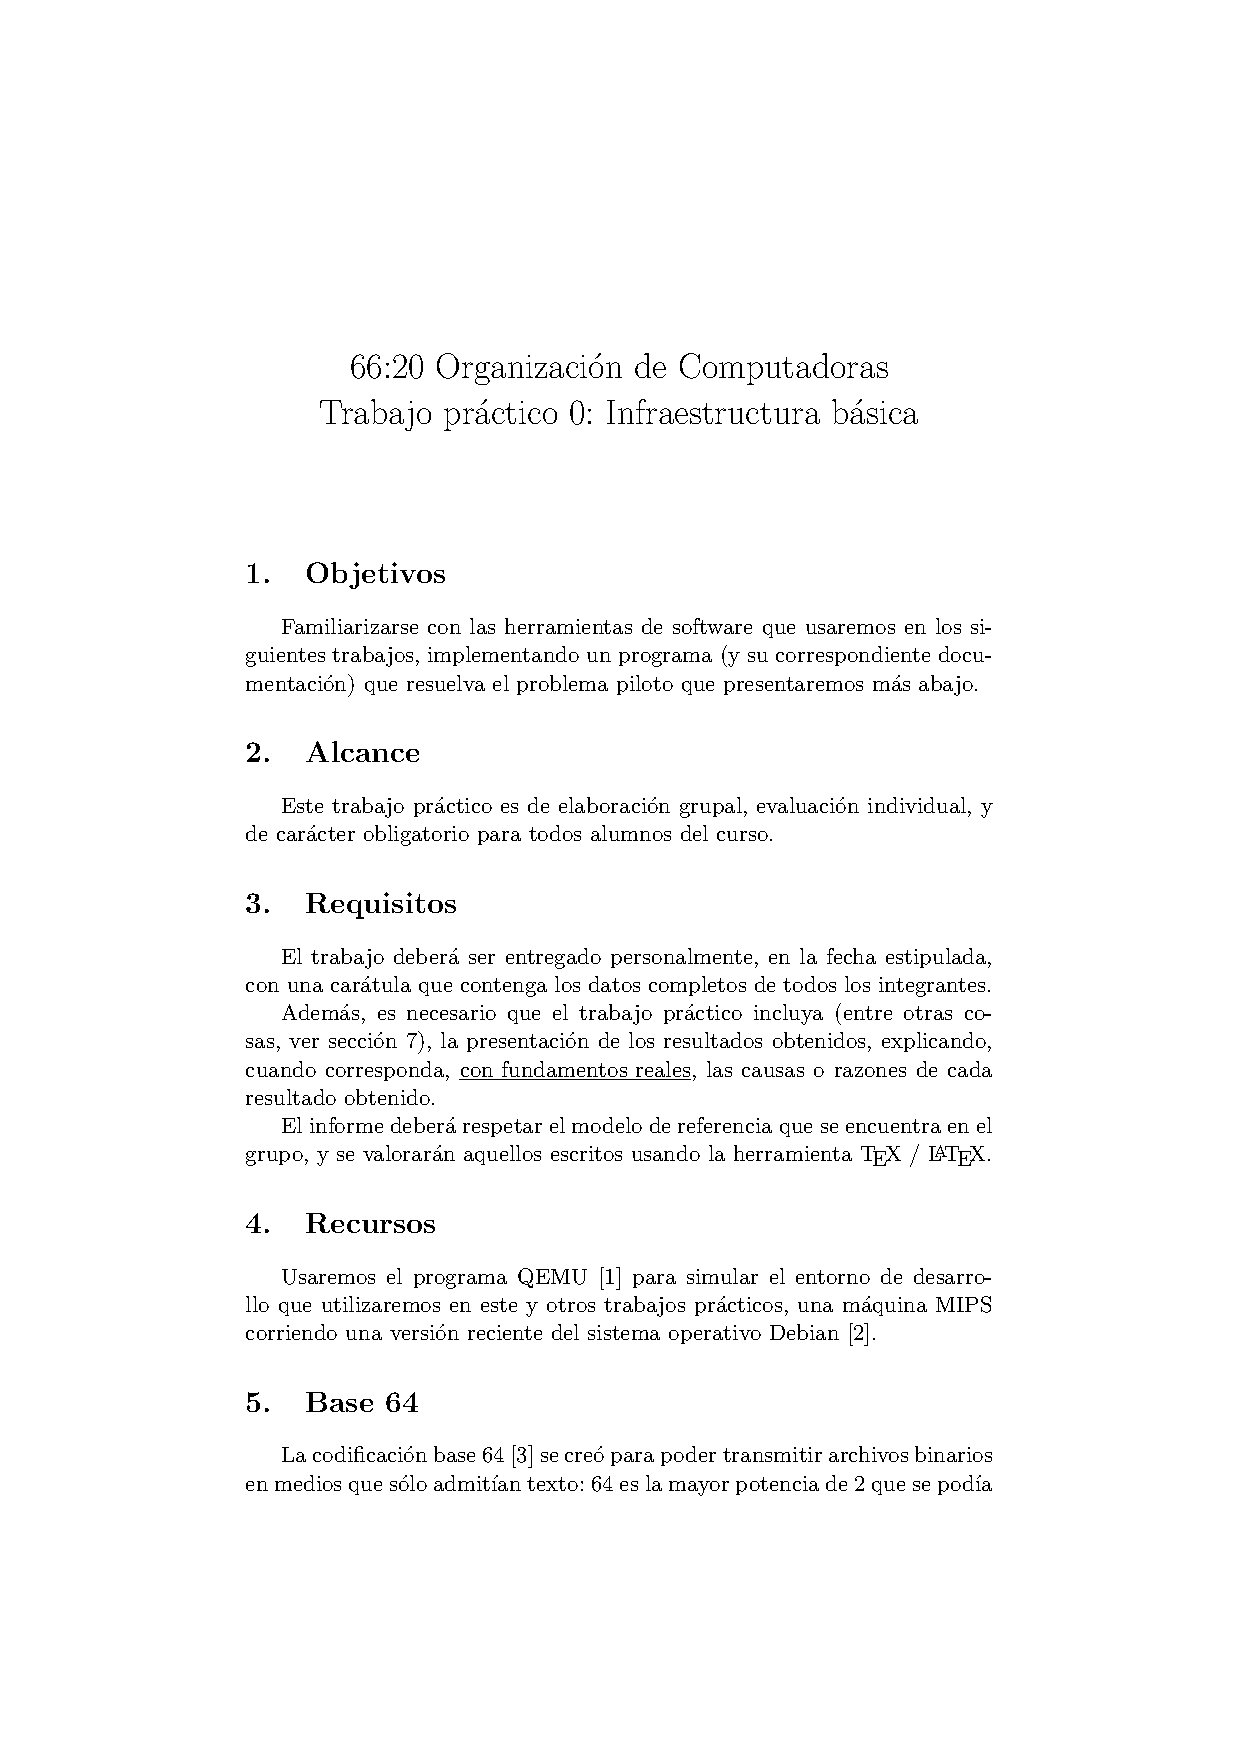
\includepdf[pages=1, scale=0.8, frame]{tp0-q2-2020.pdf}
\frame{
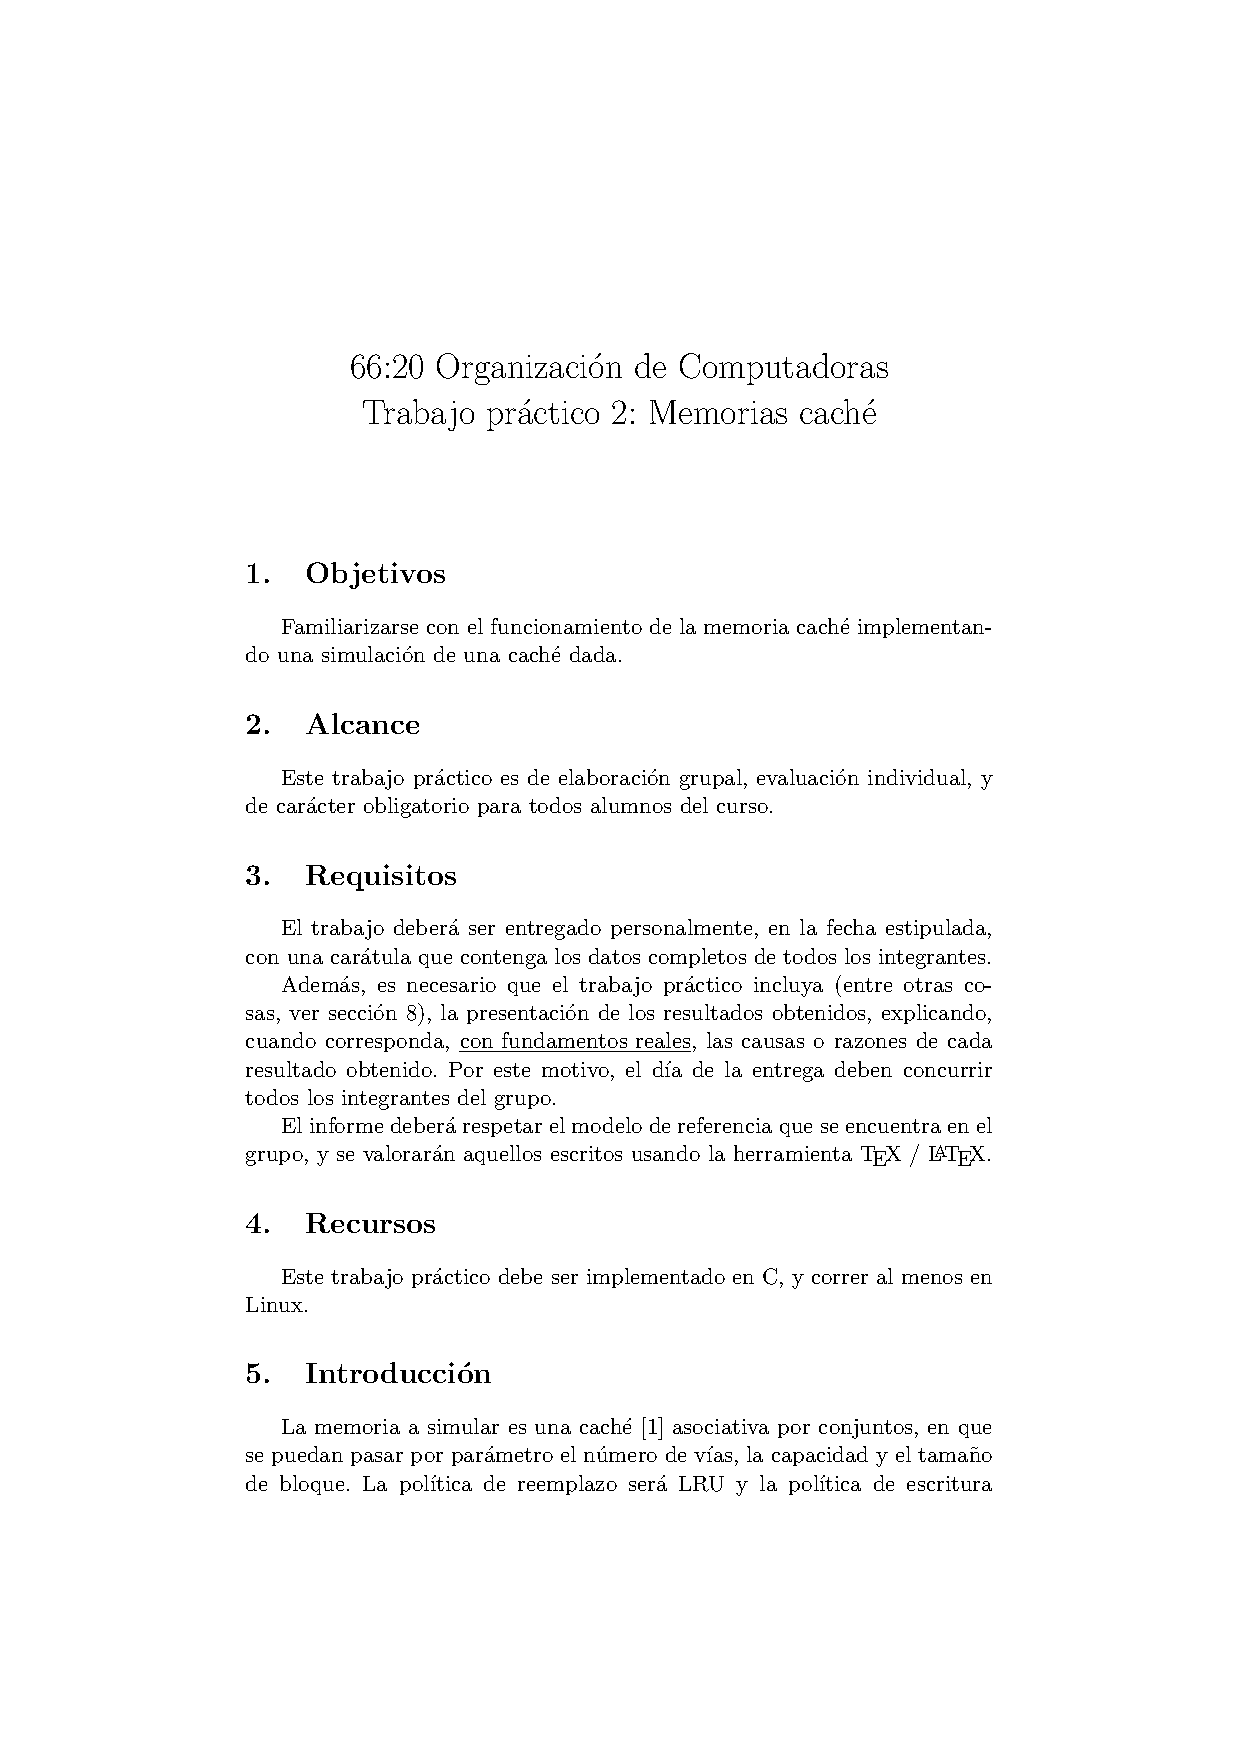
\includegraphics[height=0.93\textheight, frame]{tp2-q2-2020.pdf}
}
\includepdf[pages=2-, scale=0.8, frame]{tp2-q2-2020.pdf}
\newpage
\section{Código auxiliar}


\newpage
\begin{thebibliography}{9}


\bibitem{makefile}
\cprotect\textit{Herramienta \verb|make|}. 
\href {https://www.gnu.org/software/make/manual/make.html}{
https://www.gnu.org/software/make/manual/make.html
}



\end{thebibliography}

\end{document}